%%%%%%%%%%%%%%%%%%%%%%%%%%%%%%%%%%%%%%%%%%%%%%%%%%%%%%%%%%%%%%%%%%%%%%%%
% Escuela Politécnica Superior de la Universidad de Alicante
% Realizado por: Jose Manuel Requena Plens
% Contacto: info@jmrplens.com / Telegram:@jmrplens
%%%%%%%%%%%%%%%%%%%%%%%%%%%%%%%%%%%%%%%%%%%%%%%%%%%%%%%%%%%%%%%%%%%%%%%%

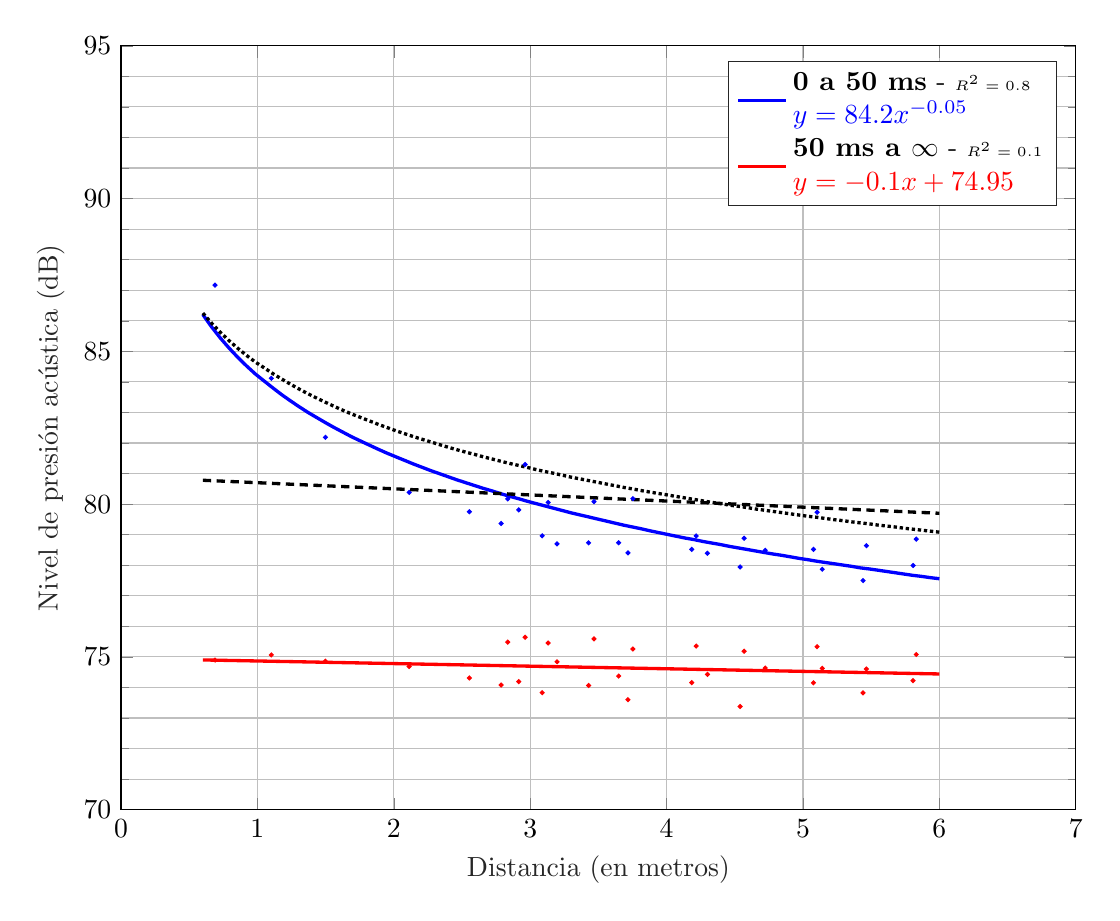
\begin{tikzpicture}

\begin{axis}[%
width=\textwidth,
height=0.8\textwidth,
at={(0\textwidth,0\textwidth)},
scale only axis,
xmin=0,
xmax=7,
xlabel style={font=\color{white!15!black}},
xlabel={Distancia (en metros)},
ymin=70,
ymax=95,
ylabel style={font=\color{white!15!black}},
ylabel={Nivel de presión acústica (dB)},
axis background/.style={fill=white},
xmajorgrids,
xminorgrids,
ymajorgrids,
yminorgrids,
minor y tick num= 4,
legend style={legend cell align=left, align=left, draw=white!15!black}
]
% Curvas EASE
\addplot[color=blue,domain=0.6:6, samples=85,line width=1.2]{84.20*x^(-0.046)};
\addlegendentry{\textbf{0 a 50 ms} - \tiny{$R^2 = 0.8$}\\$\color{blue}y = 84.2·x^{-0.05}$}

\addplot[color=red,domain=0.6:6, samples=85,line width=1.2]{-0.085*x+74.95};
\addlegendentry{\textbf{50 ms a $\infty$} - \tiny{$R^2 = 0.1$}\\$\color{red}y = -0.1·x+74.95$}

% Curvas in situ
\addplot[color=black,densely dotted,line width=1.2pt,domain=0.6:6, samples=85]{80*x^(-0.04)+4.6};
\addplot[color=black,densely dashed,line width=1.2pt,domain=0.6:6, samples=85]{-0.2*x+76.3+4.6};

% Puntos
\addplot [color=blue, only marks,mark size=0.7pt]
  table[row sep=crcr]{%
0.689492567037528	87.1678881319192\\
1.10208892563168	84.1165563459516\\
1.49833240637717	82.1847846378159\\
2.11248668634858	80.3825860852206\\
2.55409475157051	79.7499124974280\\
2.78664673039121	79.3667594554426\\
2.83511904511962	80.1691036472047\\
2.91626473421053	79.8107789453695\\
2.96261708629381	81.2962706330534\\
3.08787953132890	78.9610504227305\\
3.13169283295792	80.0551789689806\\
3.19677962956473	78.6994459080520\\
3.42820652820101	78.7315251657904\\
3.46772259559498	80.0817675993113\\
3.64836949883095	78.7344352012910\\
3.71663826596025	78.4026434296394\\
3.75311870315875	80.1768717051253\\
4.18442349673166	78.5159183345488\\
4.21685902064558	78.9590967022620\\
4.29941856534113	78.3913859061579\\
4.53878838458019	77.9424192579992\\
4.56870878914382	78.8813591154629\\
4.72298634340605	78.4870819475297\\
5.07690850813760	78.5190868467895\\
5.10367514640186	79.7316236495648\\
5.14125471067132	77.8666846191468\\
5.44027572830643	77.4974042519682\\
5.46526303118157	78.6384552124610\\
5.80710771382794	77.9892449321896\\
5.83052313261855	78.8526133593289\\
  };
  
  \addplot [color=red, only marks,mark size=0.7pt]
  table[row sep=crcr]{%
0.689492567037528	74.8956050162762\\
1.10208892563168	75.0627995710503\\
1.49833240637717	74.8603183887478\\
2.11248668634858	74.6845194840402\\
2.55409475157051	74.3092374727581\\
2.78664673039121	74.0778295615781\\
2.83511904511962	75.4835224537465\\
2.91626473421053	74.1891089179431\\
2.96261708629381	75.6398059531280\\
3.08787953132890	73.8278791984142\\
3.13169283295792	75.4544460624605\\
3.19677962956473	74.8392327702789\\
3.42820652820101	74.0635554547840\\
3.46772259559498	75.5893035097754\\
3.64836949883095	74.3702747477762\\
3.71663826596025	73.5979257690534\\
3.75311870315875	75.2568692949836\\
4.18442349673166	74.1545231838629\\
4.21685902064558	75.3525822366600\\
4.29941856534113	74.4268175950121\\
4.53878838458019	73.3756171633836\\
4.56870878914382	75.1849676241943\\
4.72298634340605	74.6336274218104\\
5.07690850813760	74.1514417003351\\
5.10367514640186	75.3339594086641\\
5.14125471067132	74.6232480840075\\
5.44027572830643	73.8223032378054\\
5.46526303118157	74.6028437546984\\
5.80710771382794	74.2216309739673\\
5.83052313261855	75.0766435298864\\
  };
\end{axis}
\end{tikzpicture}%